% -*- root: Proposal.tex -*-
\documentclass[Proposal.tex]{subfiles} 
\begin{document}
\chapter{Space-time DPG}
We summarize some completed work on space-time DPG. At the time of writing, Camellia does not officially support space-time computations, but we can fake it for 1D spatial problems by pretending the $y$-direction is time.
Complications arise when the PDE under consideration is of a different type temporally then it is spatially. 
For example, the heat equation is elliptic in space, but hyperbolic in time. 
Mathematically, this leaves traces undefined on element edges without a spatial normal component. 
Practically, this means that we have had to hack the Camellia code in order to support these ``spatial traces''.
We say that the code was ``hacked'' to indicate that we modified the code in an ``ugly'' manner in order to obtain the following results, 
but the plans are to do this in according to better software practices in the proposed work, since the current implementation is not very maintainable.

All of the following problems are run with the graph norm. 
This norm is simply defined from the adjoint of the system supplemented with $L^2$ terms to upgrade it to a full norm.

\section{Pure Convection}
The pure convection equation is 
\begin{equation}
\frac{\partial u}{\partial t}+\Div(\bfbeta u)=f\,,
\end{equation}
where $u$ is the unknown being convected, $\bfbeta$ is the convection vector, and $f$ is the source term.
The convenient thing about pure convection is that the equation is the time dimension is basically indistinguishable from the spatial dimensions. 
In fact, we can rewrite this in terms of a space-time divergence operator $\Divxt(u):=\Div(u)+\frac{\partial u}{\partial t}$:
\[
\Divxt\LRp{\vecttwo{\bfbeta}{1}u}=f\,.
\]
This means that spatially 1D space-time convection with convection vector $\alpha$ is identical to 2D steady convection with convection vector $\LRp{\alpha,1}^T$.

We derive an ultra-weak DPG formulation for pure convection with $\bfbeta=\LRp{\alpha,1}^T$. 
Multiplying by test function $v$ and integrating by parts over each element $K$, we get
\begin{equation}
-\LRp{\vecttwo{\alpha}{1}u,\Gradxt v}+\LRa{\hat t, v}=\LRp{f,v}\,,
\end{equation}
where $\hat t=\trace\LRp{\LRp{\alpha,1}^T}\cdot\bfn\,u$.

%   /$$   /$$                       /$$    
%  | $$  | $$                      | $$    
%  | $$  | $$  /$$$$$$   /$$$$$$  /$$$$$$  
%  | $$$$$$$$ /$$__  $$ |____  $$|_  $$_/  
%  | $$__  $$| $$$$$$$$  /$$$$$$$  | $$    
%  | $$  | $$| $$_____/ /$$__  $$  | $$ /$$
%  | $$  | $$|  $$$$$$$|  $$$$$$$  |  $$$$/
%  |__/  |__/ \_______/ \_______/   \___/  
%                                          
%                                          
%  
\section{Heat equation}
The simplest space-time problem we can consider where the the spatial and temporal dimensions are treated differently is the heat equation.
We start with a general $n$-dimensional spatial derivation and later simplify to spatially 1D with a few numerical experiments.

\subsection{Derivation}
Let $\Omega(t)\subset\mathbb{R}^d$ be the spatial domain with boundary $\partial\Omega$.
The heat equation is
\begin{equation}
	\frac{\partial u}{\partial t}-\epsilon\Delta u=f\,,\quad\bfx\in\Omega\,,\;t\in(t_0,T)
\end{equation}
where $u$ is unknown heat, $\epsilon$ is the diffusion scale, $f$ is the source term, $t_0$ is the start time, and $T$ is the final time.
Let $Q\subset\mathbb{R}^{d+1}$ denote the full space-time domain which is then tessellated into space-time elements $K$.

Let us proceed as usual and form a system of first order equations:
\begin{equation}
\label{eq:heatFirstOrder}
\begin{aligned}
\bfsigma-\epsilon\Grad u&=0\\
\frac{\partial u}{\partial t}-\Div\bfsigma&=f\,.
\end{aligned}
\end{equation}
Let us say that $f\in\LQ$, then we seek $u$, and $\bfsigma$ such that $u,\,\bfsigma,\,\Grad u,\,\frac{\partial u}{\partial t}-\Div\bfsigma\in\LQ$.
Notice that this is a weaker condition than saying $\frac{\partial u}{\partial t}\in\LQ$ and $\Div\bfsigma\in\LQ$.
It helps to view $\bfU:=(-\bfsigma, u)$ as a group variable in space-time. 
Then the last condition is telling us that $\Divxt\bfU\in\LQ$, or that $\bfU\in\HdivQ$.
That is to say the normal component $-\bfsigma\cdot\bfn_x+u\cdot n_t$ (which we call the flux) is continuous across element faces, 
where $\bfn=(\bfn_x,n_t)^T$ is the full space-time normal vector for element $K$.
Now consider the condition that $\Grad u\in\LQ$.
This implies that $u$ lives in a tensor product space of $H^1$ spatially and $L^2$ temporally and that
$u\cdot n_t$ is continuous on element faces where $n_t$ is nonzero; we call this the spatial trace.

Now that we understand which Sobolev spaces $u$ and $\bfsigma$ live in, we can proceed with a derivation of the space-time DPG formulation for this problem.
We multiply the first equation in \eqref{eq:heatFirstOrder} by test function $\bftau$ and the second by $v$. Then we integrate by parts over each element:
\begin{equation}
\label{eq:heatBF}
	\begin{aligned}
		\LRp{\bfsigma,\bftau}+\epsilon\LRp{u,\Div\bftau}-\LRa{\hat u,\tau_n}&=0\\
		-\LRp{u,\frac{\partial v}{\partial t}}+\LRp{\bfsigma,\Grad v}-\LRa{\hat t,v}&=\LRp{f,v}\,,
	\end{aligned}
\end{equation}
where $\hat u$ is the spatial trace and $\hat t$ is the flux.
The second equation could alternatively be written in terms of the group variable $\bfU$:
\begin{equation}
\label{heatBFAlt}
-\LRp{\bfU,\Gradxt v}-\LRa{\hat t,v}=\LRp{f,v}\,.
\end{equation}
This alternate version emphasizes the definition of the flux: $\hat t=\trace\LRp{-\bfsigma}\cdot\bfn_x+\trace{(u)}\cdot n_t$.
From \eqref{eq:heatBF} and \eqref{heatBFAlt} it is clear that $\bftau\in\HdivK$ where the divergence is taken only over spatial directions, and $v\in\HOneK$.
Figure \ref{fig:heatMesh} illustrates the support for the fluxes and spatial traces. Notice that the fluxes live on all element boundaries, while the spatial traces only live on ``non-horizontal'' edges.

\begin{figure}[h!]
\begin{tikzpicture}[line cap=round,line join=round,>=triangle 45,x=2.0cm,y=2.0cm]
\clip(-0.7,-1.01) rectangle (5.27,2.29);
\draw (0,2)-- (0,0);
\draw (0,0)-- (1,0);
\draw (1,0)-- (4,0);
\draw (4,0)-- (5,0);
\draw (5,0)-- (5,2);
\draw (5,2)-- (3,2);
\draw (3,2)-- (2,2);
\draw (2,2)-- (0,2);
\draw (1,0)-- (1.5,1);
\draw (1.5,1)-- (2,2);
\draw (1.5,1)-- (3.5,1);
\draw (3,2)-- (3.5,1);
\draw (3.5,1)-- (4,0);
\draw (-0.21,0.9) node[anchor=south west] {$\hat u$};
\draw (4.82,0.9) node[anchor=south west] {$\hat u$};
\draw (3.5,0.45) node[anchor=south west] {$\hat u$};
\draw (1.0,0.45) node[anchor=south west] {$\hat u$};
\draw (1.5,1.4) node[anchor=south west] {$\hat u$};
\draw (3.0,1.4) node[anchor=south west] {$\hat u$};
\draw (0.05,0.9) node[anchor=south west] {$\hat t$};
\draw (1.40,0.45) node[anchor=south west] {$\hat t$};
\draw (3.79,0.45) node[anchor=south west] {$\hat t$};
\draw (2.47,1.0) node[anchor=south west] {$\hat t$};
\draw (3.33,1.4) node[anchor=south west] {$\hat t$};
\draw (1.89,1.4) node[anchor=south west] {$\hat t$};
\draw (5.07,0.9) node[anchor=south west] {$\hat t$};
\draw (4.44,0.0) node[anchor=south west] {$\hat t$};
\draw (2.46,0.0) node[anchor=south west] {$\hat t$};
\draw (0.45,0.0) node[anchor=south west] {$\hat t$};
\draw (2.44,1.7) node[anchor=south west] {$\hat t$};
\draw (0.76,1.7) node[anchor=south west] {$\hat t$};
\draw (4.21,1.7) node[anchor=south west] {$\hat t$};
\draw [->] (-0.5,-0.5) -- (-0.5,0);
\draw [->] (-0.5,-0.5) -- (0,-0.5);
\draw (-0.54,0.29) node[anchor=north west] {$t$};
\draw (0.07,-0.35) node[anchor=north west] {$x$};
\end{tikzpicture}
\caption{Support of flux and spatial trace variables}
\label{fig:heatMesh}
\end{figure}

\subsection{Problems considered}
If we consider a domain $\Omega=[0,1]^2$ with an initial condition of $u=\cos(2\pi x)$ with zero flux conditions at the boundaries,
the exact solution is
\begin{equation*}
	u=\cos(2\pi x)e^{-4*\pi^2\epsilon t}\,.
\end{equation*}
We ran this with $\epsilon=10^{-2}$ on a sequence of uniform meshes and $p=2$ for the field representation of $u$. 
We were able to achieve the expected third order convergence as demonstrated in Figure \ref{fig:spaceTimeHeatConvergence}.

\begin{figure}[!ht]
	\centering
	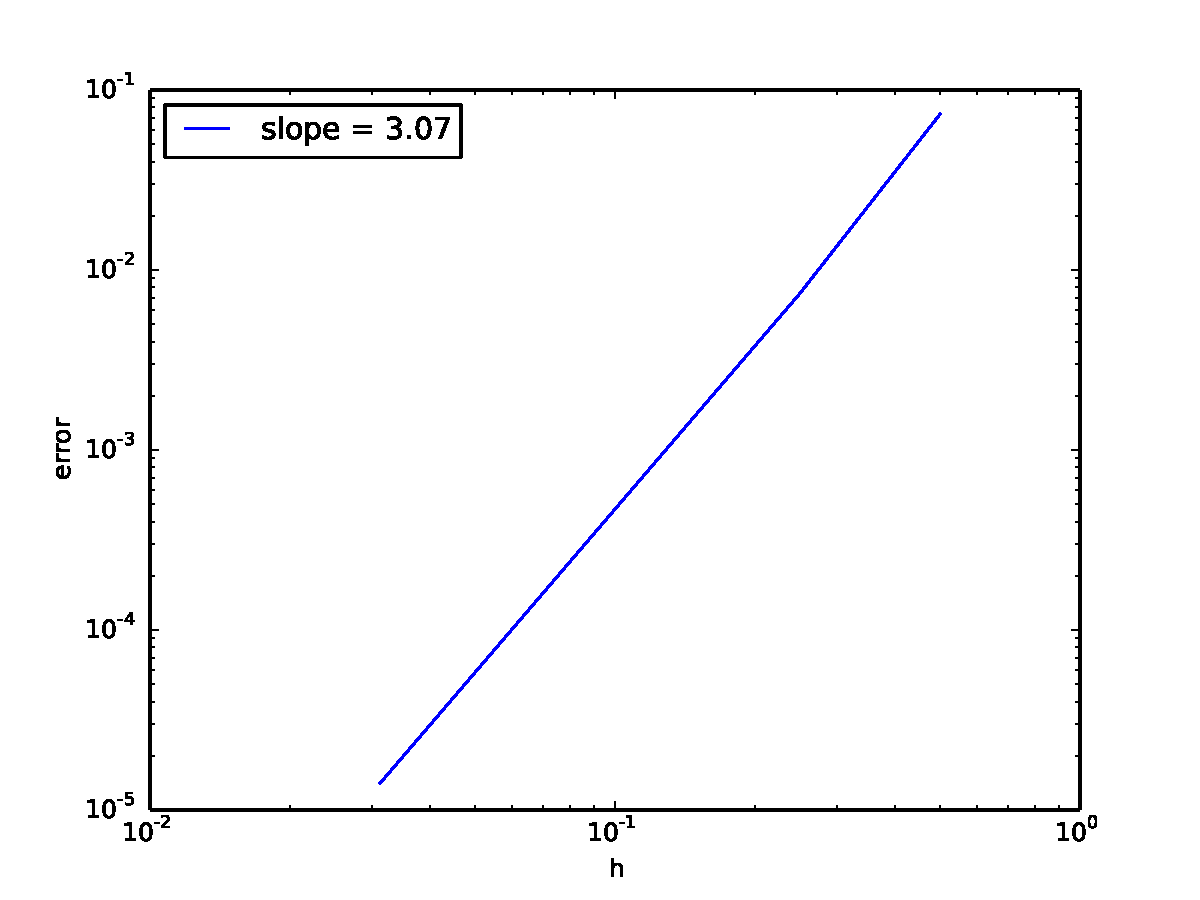
\includegraphics[width=0.7\textwidth]{SpaceTimeHeat/convergence}
	\caption{$L^2$ convergence of $u$ for the space-time heat equation}
	\label{fig:spaceTimeHeatConvergence}
\end{figure}

In order to demonstrate local space-time adaptivity we consider one more problem for the heat equation. 
On the same domain, and with the same boundary conditions as the previous example, we let the initial heat distribution be zero.
Then between $t=0.25$ and $t=0.5$ we turn on a pulse source term of one on $0.375\leq x\leq 0.625$. 
Starting from an initial mesh of $4x4$, we adaptively refine four times and obtain the results in Figure \ref{fig:spaceTimeHeatPulse}.
Notice that $\hat u$ in Figure \ref{fig:spaceTimeHeatuhat} only lives on vertical edges as was discussed earlier.
Also notice that the full mesh shown in Figure \ref{fig:spaceTimeHeatfhat} automatically adapts spatially and temporally to where features are rapidly changing. 

\begin{figure}[ht]
\centering
\begin{subfigure}[t]{0.45\textwidth}
\centering
\includegraphics[width=\textwidth]{SpaceTimeHeat/PulseSource/u.png}
\caption{$u$}
\label{fig:spaceTimeHeatu}
\end{subfigure}
\begin{subfigure}[t]{0.45\textwidth}
\centering
\includegraphics[width=\textwidth]{SpaceTimeHeat/PulseSource/sigma.png}
\caption{$\sigma$}
\label{fig:spaceTimeHeatsigma}
\end{subfigure}
\begin{subfigure}[t]{0.45\textwidth}
\centering
\includegraphics[width=\textwidth]{SpaceTimeHeat/PulseSource/uhat.png}
\caption{$\hat u$}
\label{fig:spaceTimeHeatuhat}
\end{subfigure}
\begin{subfigure}[t]{0.45\textwidth}
\centering
\includegraphics[width=\textwidth]{SpaceTimeHeat/PulseSource/fhat.png}
\caption{$\hat t$}
\label{fig:spaceTimeHeatfhat}
\end{subfigure}
\caption{Pulsed space-time heat problem after 4 refinements}
\label{fig:spaceTimeHeatPulse}
\end{figure}

%    /$$$$$$                       /$$$$$$                      /$$                    
%   /$$__  $$                     /$$__  $$                    |__/                    
%  | $$  \__/  /$$$$$$  /$$$$$$$ | $$  \__/ /$$   /$$  /$$$$$$$ /$$  /$$$$$$  /$$$$$$$ 
%  | $$       /$$__  $$| $$__  $$| $$$$    | $$  | $$ /$$_____/| $$ /$$__  $$| $$__  $$
%  | $$      | $$  \ $$| $$  \ $$| $$_/    | $$  | $$|  $$$$$$ | $$| $$  \ $$| $$  \ $$
%  | $$    $$| $$  | $$| $$  | $$| $$      | $$  | $$ \____  $$| $$| $$  | $$| $$  | $$
%  |  $$$$$$/|  $$$$$$/| $$  | $$| $$      |  $$$$$$/ /$$$$$$$/| $$|  $$$$$$/| $$  | $$
%   \______/  \______/ |__/  |__/|__/       \______/ |_______/ |__/ \______/ |__/  |__/
%                                                                                      
%                                                                                      
%        
\section{Convection-diffusion}
Transient convection-diffusion is identical to the heat equation with the addition of a convective term:
\begin{equation*}
\frac{\partial u}{\partial t}+\Div(\bfbeta u)-\epsilon\Delta u=f\,.
\end{equation*}
The $d$-dimensional transient convection-diffusion equations could be viewed as a $d+1$ steady convection-diffusion problem with zero diffusion in the time direction.

\subsection{Derivation}
As a first order system, this is
\begin{equation}
\label{eq:confusionFirstOrder}
\begin{aligned}
\bfsigma-\epsilon\Grad u&=0\\
\frac{\partial u}{\partial t}+\Div\LRp{\bfbeta u-\bfsigma}&=f\,.
\end{aligned}
\end{equation}
We can view the second equation as a full space-time divergence on group variable $\bfU:=\LRc{\bfbeta u-\bfsigma,u}$ as before:
\begin{equation}
	\Divxt\LRp{\bfU}=f\,.
\end{equation}
Multiplying \eqref{eq:confusionFirstOrder} by test functions, and integrating by parts over each element, we obtain the following bilinear form:
\begin{equation}
\label{eq:confusionBF}
	\begin{aligned}
		\LRp{\bfsigma,\bftau}+\epsilon\LRp{u,\Div\bftau}-\LRa{\hat u,\tau_n}&=0\\
		-\LRp{u,\frac{\partial v}{\partial t}}-\LRp{\bfbeta u,\Grad v}+\LRp{\bfsigma,\Grad v}-\LRa{\hat t,v}&=\LRp{f,v}\,,
	\end{aligned}
\end{equation}
where now $\hat t=\trace\LRp{\bfbeta u-\bfsigma}\cdot\bfn_x+\trace(u)\cdot n_t$, and $\hat u$ is as before. Our test functions, $\bftau$ and $n$ live in the same spaces as for the heat equation.

\subsection{Problems considered}
Since space-time convection-diffusion is identical the heat equation with the addition of a convective term, we only pursue one numerical experiment to demonstrate that everything works as expected. 
This problem is inspired by the previous heat problem with the spatial domain extended to prevent the convected heat from impinging on the right wall.
It might be interesting to impose a zero boundary condition on $\hat u$ and watch a boundary layer build up on the right wall, 
but instead we enforce a zero flux condition and content ourselves with the inner layer that forms around the source pulse.
This is an arbitrary requirement necessitated by the ``hackish'' nature of this code.
We haven't taken the time to allow enforcement of Dirichlet boundary conditions on spatial fluxes, and since the code in this state was intended to be short-lived, it doesn't make sense to invest too heavily in adding features. 
Thus we enforce zero flux conditions on both walls as before. 
For this problem, the domain extends from $[0,1.5]\times[0,1]$ with the pulse occurring at $[0.25,0.5]\times[0.25,0.5]$.

\begin{figure}[ht]
\centering
\begin{subfigure}[t]{0.45\textwidth}
\centering
\includegraphics[width=\textwidth]{SpaceTimeConfusion/u.png}
\caption{$u$}
\label{fig:spaceTimeConfusionu}
\end{subfigure}
\begin{subfigure}[t]{0.45\textwidth}
\centering
\includegraphics[width=\textwidth]{SpaceTimeConfusion/sigma.png}
\caption{$\sigma$}
\label{fig:spaceTimeConfusionsigma}
\end{subfigure}
\begin{subfigure}[t]{0.45\textwidth}
\centering
\includegraphics[width=\textwidth]{SpaceTimeConfusion/uhat.png}
\caption{$\hat u$}
\label{fig:spaceTimeConfusionuhat}
\end{subfigure}
\begin{subfigure}[t]{0.45\textwidth}
\centering
\includegraphics[width=\textwidth]{SpaceTimeConfusion/fhat.png}
\caption{$\hat t$}
\label{fig:spaceTimeConfusionfhat}
\end{subfigure}
\caption{Space-time convection-diffusion problem after 4 refinements}
\label{fig:spaceTimeConfusion}
\end{figure}

%   /$$$$$$$                                                             
%  | $$__  $$                                                            
%  | $$  \ $$ /$$   /$$  /$$$$$$   /$$$$$$   /$$$$$$   /$$$$$$   /$$$$$$$
%  | $$$$$$$ | $$  | $$ /$$__  $$ /$$__  $$ /$$__  $$ /$$__  $$ /$$_____/
%  | $$__  $$| $$  | $$| $$  \__/| $$  \ $$| $$$$$$$$| $$  \__/|  $$$$$$ 
%  | $$  \ $$| $$  | $$| $$      | $$  | $$| $$_____/| $$       \____  $$
%  | $$$$$$$/|  $$$$$$/| $$      |  $$$$$$$|  $$$$$$$| $$       /$$$$$$$/
%  |_______/  \______/ |__/       \____  $$ \_______/|__/      |_______/ 
%                                 /$$  \ $$                              
%                                |  $$$$$$/                              
%                                 \______/   
\section{Burgers'}

\subsection{Derivation}

\subsection{Problems considered}

%    /$$$$$$                                                                            /$$ /$$       /$$          
%   /$$__  $$                                                                          |__/| $$      | $$          
%  | $$  \__/  /$$$$$$  /$$$$$$/$$$$   /$$$$$$   /$$$$$$   /$$$$$$   /$$$$$$$  /$$$$$$$ /$$| $$$$$$$ | $$  /$$$$$$ 
%  | $$       /$$__  $$| $$_  $$_  $$ /$$__  $$ /$$__  $$ /$$__  $$ /$$_____/ /$$_____/| $$| $$__  $$| $$ /$$__  $$
%  | $$      | $$  \ $$| $$ \ $$ \ $$| $$  \ $$| $$  \__/| $$$$$$$$|  $$$$$$ |  $$$$$$ | $$| $$  \ $$| $$| $$$$$$$$
%  | $$    $$| $$  | $$| $$ | $$ | $$| $$  | $$| $$      | $$_____/ \____  $$ \____  $$| $$| $$  | $$| $$| $$_____/
%  |  $$$$$$/|  $$$$$$/| $$ | $$ | $$| $$$$$$$/| $$      |  $$$$$$$ /$$$$$$$/ /$$$$$$$/| $$| $$$$$$$/| $$|  $$$$$$$
%   \______/  \______/ |__/ |__/ |__/| $$____/ |__/       \_______/|_______/ |_______/ |__/|_______/ |__/ \_______/
%                                    | $$                                                                          
%                                    | $$                                                                          
%                                    |__/    
\section{Compressible Navier-Stokes}

\subsection{Derivation}

\subsection{Problems considered}

\section{Time-slabs vs full-time}
\end{document}